\subsection{Application Features}


\subsubsection{Graphic User Interface with PyTorch}
 
The goal of our programming project is to develope  a Python-based GUI (Graphical User Interface) 
that uses PyTorch scientific tools and  Libraries which will be an open-source deep learning frameworks such as Expresso  for  Caffe,  NVidia  DIGITS  for  Theano,  Caffe,  Torch  and  Tensorflow.   Even though there are lot  of  graphical  user
interface which provide numerous tools for deep learning frameworks are available but unfortunately they are not
compatible with PyTorch Library at the moment we begin this project. Therefore, the alternative we propose is
an application that will be an interface for PyTorch and gives the abilities to use all the deep learning features
provided by the Pytorch framework.
Our application goal is to provides interesting features with manipulation of neural network. It will also integrate
Jupyter-Notebook thus user could expereience live coding, graph computation and specifically neural network
vizualisations.

\begin{figure}[!ht]
    \center 
    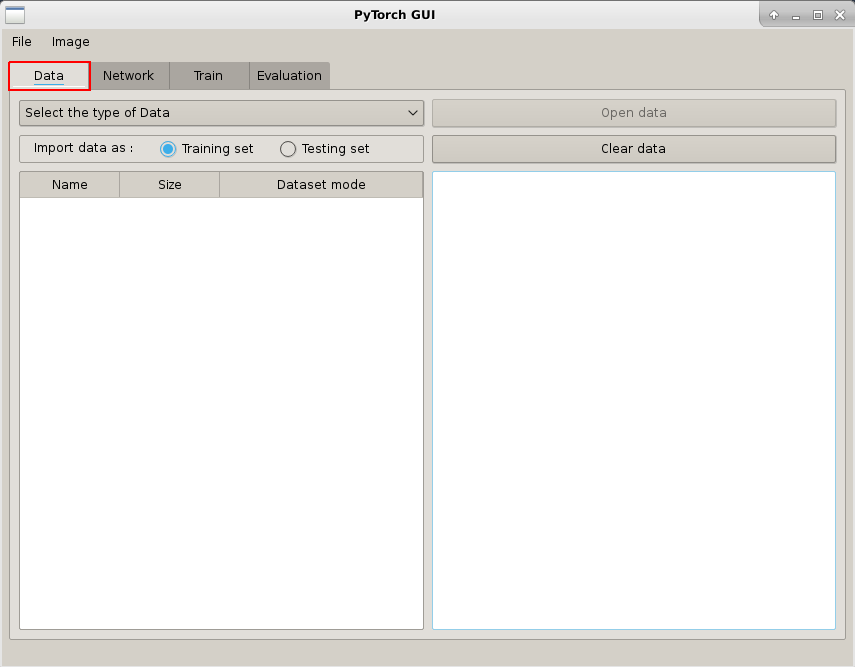
\includegraphics[scale=0.5]{figures/app_screen_shoots/Data_tab.png}
    \caption{Data Tab}
\end{figure}

\begin{figure}[!ht]
    \center
    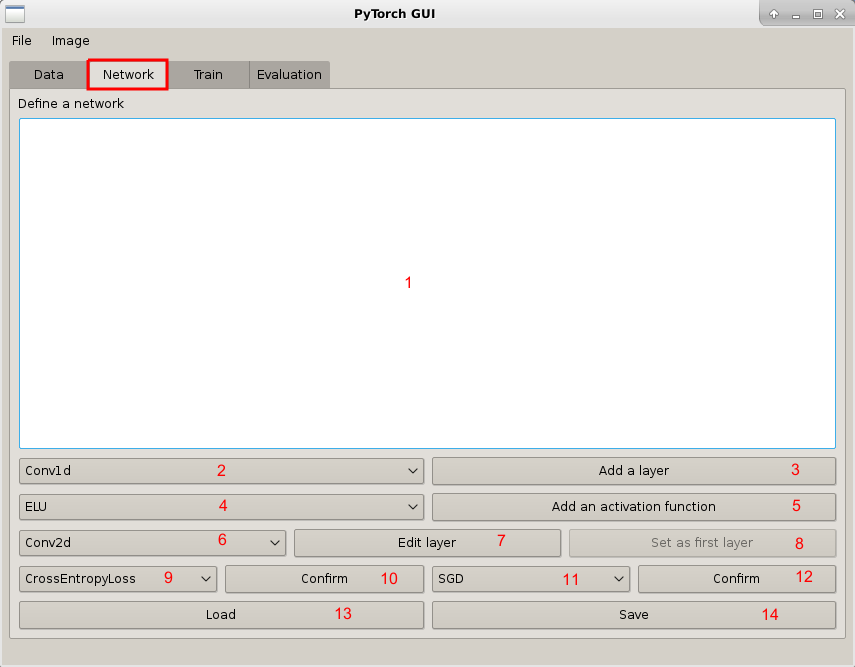
\includegraphics[scale=0.5]{figures/app_screen_shoots/Network_tab.png}
    \caption{Network Tab}
\end{figure}

\begin{figure}[!ht]
    \center
    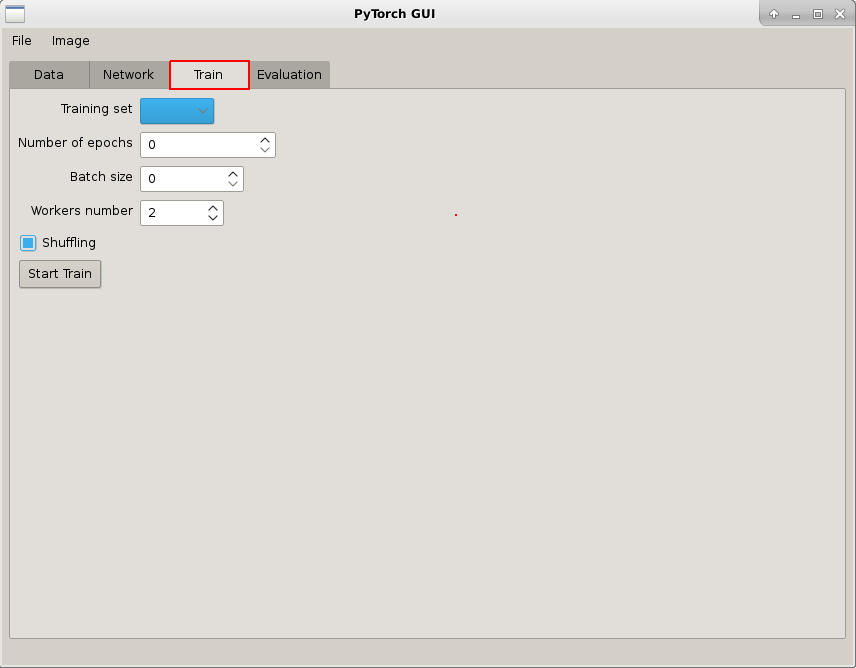
\includegraphics[scale=0.5]{figures/app_screen_shoots/Train_tab.png}
    \caption{Train Tabe}
\end{figure}

\begin{figure}[!ht]
    \center
    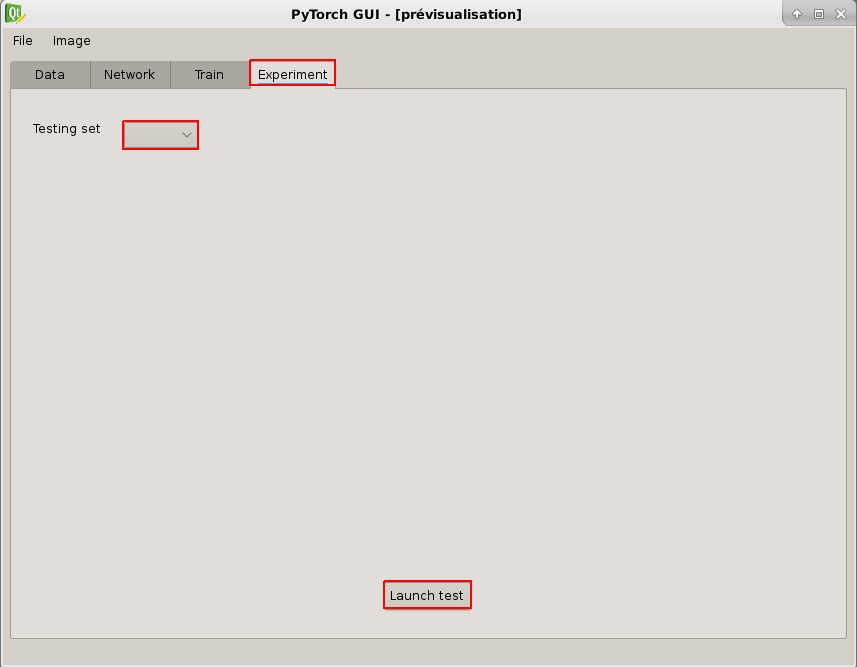
\includegraphics[scale=0.5]{figures/app_screen_shoots/Experiment_tab.png}
    \caption{Experiment Tabe}
\end{figure}


\\\
\\\
\\\
\\\
\\\
\\\